\documentclass{article}
\usepackage{graphicx} % Required for inserting images
\graphicspath{ {./img/} }

\usepackage{hyperref}
\usepackage{amsmath}
\usepackage{amsfonts}
\usepackage{physics}

\title{Introduction to Quantum Information and Computing - Lecture 6}
\author{Shrikara A, Arnav Negi, Kriti Gupta, Manav Shah, Mohammed Shamil,\\ Shiven Sinha, Swayam Agarwal, Vineeth Bhat, Yash Adivarekar} % add contributors
\date{24th January, 2023}

\begin{document}


    \pagenumbering{gobble}
    \maketitle
    \vfill
    \tableofcontents
    \newpage
    \pagenumbering{arabic}

% Equations:
%     \begin{gather*}
%      \mathcal{N} _{A \rightarrow B} : \mathcal{B}(\mathcal{H _{A}}) \xrightarrow \mathcal{B}(\mathcal{H _{B}}) 
%     \end{gather*}
        % \begin{center}
        %     \((\mathcal{H _{A}})\) = Hilbert space of input system, 
            
        %     \( (\mathcal{B}) \) = Set of bounded operators  
        % \end{center}

% \medskip
%         \small
        % \normalsize
        % \textbf{Super Operator}
        
        % \subsection{Properties of Quantum Channel}


\section{General Quantum Circuits}
Elementary gates can be composed into bigger quantum circuits.

This can be done in two ways:
\begin{enumerate}
    \item Tensor product
    \item Ordinary matrix product
\end{enumerate}

\subsection{Tensor Product}
Combination of gates applied to different registers.

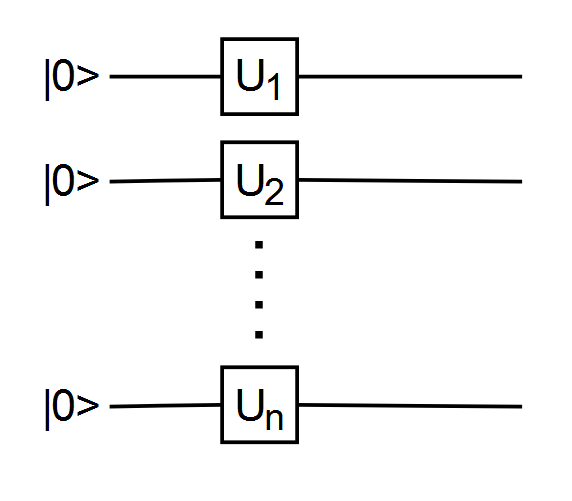
\includegraphics[scale=0.5]{q1.png}

\begin{center}
$    U_{1} \ket{0} \otimes U_{2} \ket{0} ... U_{n} \ket{0}
    = (U_{1} \otimes U_{2} ... \otimes U_{n}) \ket{0...0}$


    $= U^{\otimes n} \ket{0^{n}}$ when $U_{i}=U \forall i$
    
\end{center}

$(U_{1} \otimes U_{2} ... \otimes U_{n}) $ is a $2^{n}$ dimension unitary.

\subsection{Ordinary Matrix Product}
Combination of gates applied to same register.

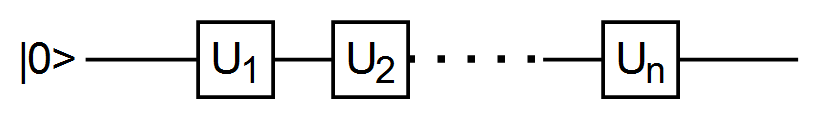
\includegraphics[scale=0.5]{q2.png}

Output, $\ket{\psi} = (U_{n}...U_{1})\ket{0}$

Here, for all $U$, dim = $2 \times 2 $ (if all $U_{i}s$ are single qubit)

\section{Cost of Quantum Circuits}

\begin{enumerate}
    \item Gate complexity
    \item Depth complexity 
    \item Query complexity
\end{enumerate}
\subsection{Query Complexity}
Query complexity is decided by number of queries made to a blackbox, $U_{f}$.

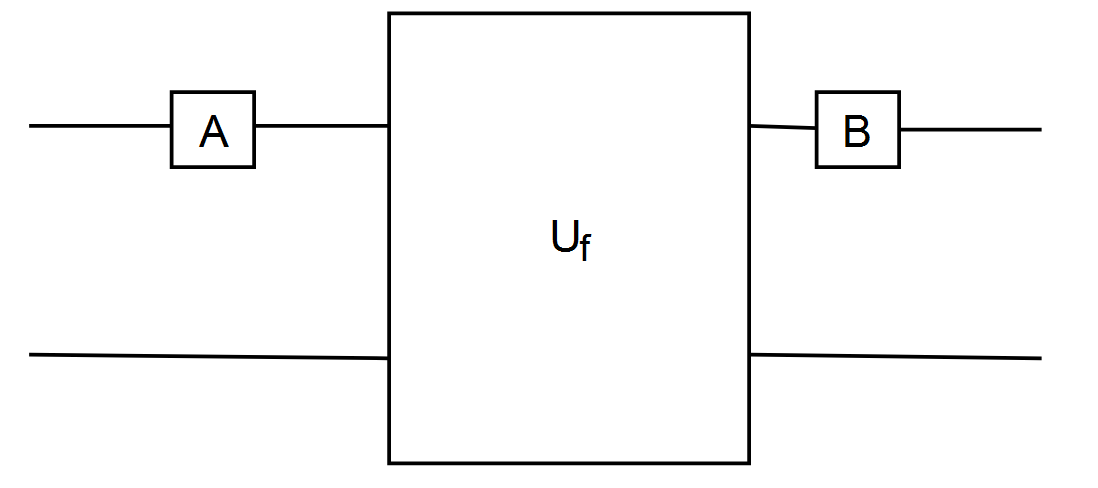
\includegraphics[scale=0.5]{q3.png}

Gates added before and after the blackbox to prepare desired input/output state do not affect the complexity. 

\section{State produced by Hadamard Gate}

\subsection{Single Hadamard gate}

\begin{gather*}
    H = \frac{1}{\sqrt{2}} 
    \begin{pmatrix}
    1 & 1\\
    1 & -1
    \end{pmatrix}
\end{gather*}
\begin{gather*}
    H \ket{0} = \frac{1}{\sqrt{2}} (\ket{0}+\ket{1})
\end{gather*}
\begin{gather*}
    H \ket{1} = \frac{1}{\sqrt{2}} (\ket{0}-\ket{1})
\end{gather*}

when $x \in \{0, 1\}$,

\begin{gather*}
    H \ket{x} = \frac{1}{\sqrt{2}} (\ket{0}+ (-1)^{x}\ket{1})
    =  \frac{1}{\sqrt{2}} \sum \limits _{z \in \{0,1\}} (-1)^{xz} \ket{z}
\end{gather*}

\subsection{N Hadamard gates}
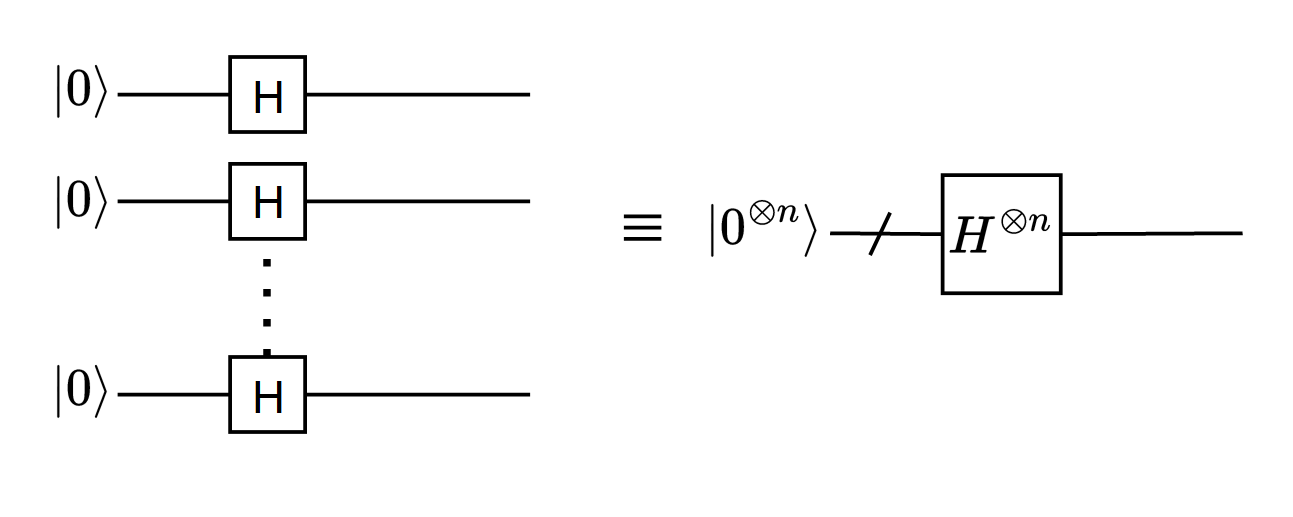
\includegraphics[scale=0.5]{q4.png}
$H^{\otimes n} = H \otimes H ... \otimes H$

\begin{align*}
Output &= \ket{+^{\otimes n}}\\
&= \frac{1}{\sqrt{2}^{n}} (\ket{0} + \ket{1}) \otimes \frac{1}{\sqrt{2}} (\ket{0} + \ket{1}) ... \otimes \frac{1}{\sqrt{2}} (\ket{0} + \ket{1}) \\
&= \frac{1}{\sqrt{2}^{n}} (\ket{0...000} + \ket{0...001} + \ket{0...010} ...)\\
&= \frac{1}{\sqrt{2}^{n}} \sum (\text{basis of n qubits)}\\\\
H^{\otimes n} \ket{0^{\otimes n}} &= \frac{1}{\sqrt{2}^{n}} \sum \limits _{z \in {0,1}^{n}} \otimes \ket{z}\\\\
H^{\otimes n} \ket{x} &= \frac{1}{\sqrt{2}^{n}} \sum \limits _{z \in {0,1}^{n}} \otimes (-1)^{x \cdot z}\ket{z}
\end{align*}

\section{Universality of Quantum Gates}
Can any U be decomposed into a combination of unitaries/gates from some finite set?

\begin{enumerate}
    \item {CNOT, all single qubit gates} $\equiv$ universal set for QC $\xrightarrow{}$ but, not finite
    \item{CNOT, H, T} = G \} Good approximation for any quantum gate.
\end{enumerate}

\subsection{Solovay-Kitaev Theorem}
\begin{itemize}
    \item Uses G, and each of the gates' inverse
\end{itemize}

\subsubsection{1-2 Qubit}
It is possible to approximate any unitary (gate) in one or two qubits upto an error $\epsilon$ by using only $O(polylog(\frac{1}{\epsilon})$ gates from G.

$\norm{U \ket{\psi} - U_{m} U_{m-1} ... U_{1} \ket{\psi}} \leq \epsilon$

Where $U$ is the matrix being approximated and each $U_{i} \in G$ and $m \in {polylog(\frac{1}{\epsilon})}$

\subsubsection{t-Gate}
Any '$t$' gate quantum circuit can be $\epsilon$-approximated by only $O(t \cdot polylog(\frac{1}{\epsilon})$ gates from G

\section{Quantum Parallelism}
\begin{itemize}
    \item Quantum circuits can be applied to multiple/all states in one query.
    \item But, output would still be of no use until we apply appropriate transformations to separate the outputs.
\end{itemize} 

E.g., Consider a classical circuit that computes 
\begin{align*}
    f: \{0, 1\}^{n} \rightarrow \{0, 1\}
\end{align*}
We need to run this $2^{n}$ times (once for each input) to find output for each input.
\medskip
Converting it to a quantum circuit but replacing gates with reversible unitaries,
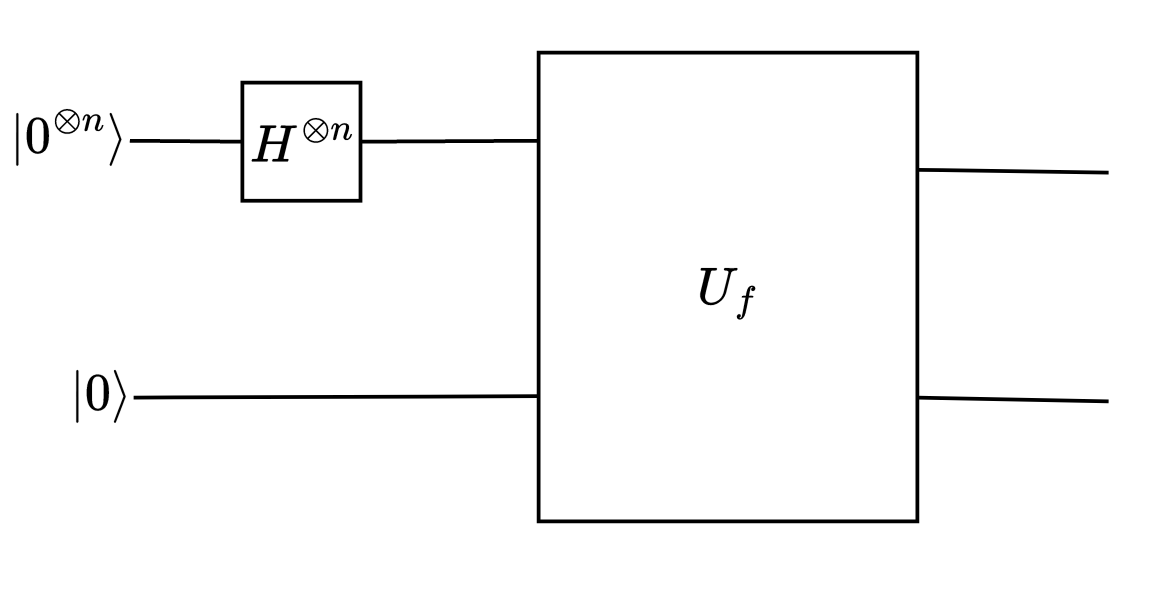
\includegraphics[scale=0.5]{q5.png}
$Output, \ket{\psi} = \frac{1}{\sqrt{2}^{n}} \sum \limits _{z \in \{0, 1\}^{n}} \ket{z} \ket{f(\ket{z})} $

\end{document}